\vspace{-0.1in}
\subsection{Problem Formulation}\label{sec:formulation}
We focus on predictive inference of a time-varying stochastic process, whose mean $f$ evolves temporally via $f_{\tindex+1} \sim \mathbb{F}(f_{\tindex},\eta_{\tindex})$, where $\mathbb{F}$ is a distribution varying with time $\tindex$ and exogenous inputs $\eta$. Our approach builds on the fact that in several cases, temporal evolution can be hierarchically separated from spatial functional evolution. A classical and quite general example of this is the \emph{abstract evolution equation} (AEO), which can be defined as the evolution of a function $\banachfunc$ embedded in a Banach space $\banachspace$: $\dot{\banachfunc}(t) = \banachop\banachfunc(t)$, subject to $\banachfunc(0)= \banachfunc_0$, and $\banachop:\banachspace\to\banachspace$ determines spatiotemporal transitions of $\banachfunc\in\banachspace$ \cite{brezis2010functional}. This model of spatiotemporal evolution is very general (AEOs, for example, model many PDEs), but working in Banach spaces can be computationally taxing.  A simple way to make the approach computationally feasible is to place restrictions on $\banachspace$: in particular, we restrict the sequence $f_{\tindex}$ to lie in a Reproducing Kernel Hilbert Space (RKHS), the theory of which provides powerful tools for generating flexible classes of functions with relative ease \cite{RasmussenWilliams2005}.
In a kernel-based model, $\kernel:\dom\times\dom\to\R$ is a positive-definite Mercer kernel on a domain $\dom$ that models the covariance between any two points in the input space,  
and implies the existence of a smooth map $\fmap:\dom\to\fspace$, where $\fspace$ is an RKHS with the property $\kernel(x,y) = \Kiprod{x}{y}$. The key insight behind the proposed model is that spatiotemporal evolution in the input domain corresponds to temporal evolution of the mixing weights of a kernel model alone in the functional domain. Therefore, $f_{\tindex}$ can be modeled by tracing the evolution of its mean embedded in a RKHS using switched ordinary differential equations (ODE) when the evolution is continuous, or switched difference equations when it is discrete (Figure \ref{fig:hilbert_evolution}). 
The advantage of this approach is that it allows us to utilize powerful ideas from systems theory for deriving necessary and sufficient conditions for spatiotemporal monitoring. 

\begin{figure}
	\centering
	\begin{minipage}{0.45\textwidth}
	\centering
	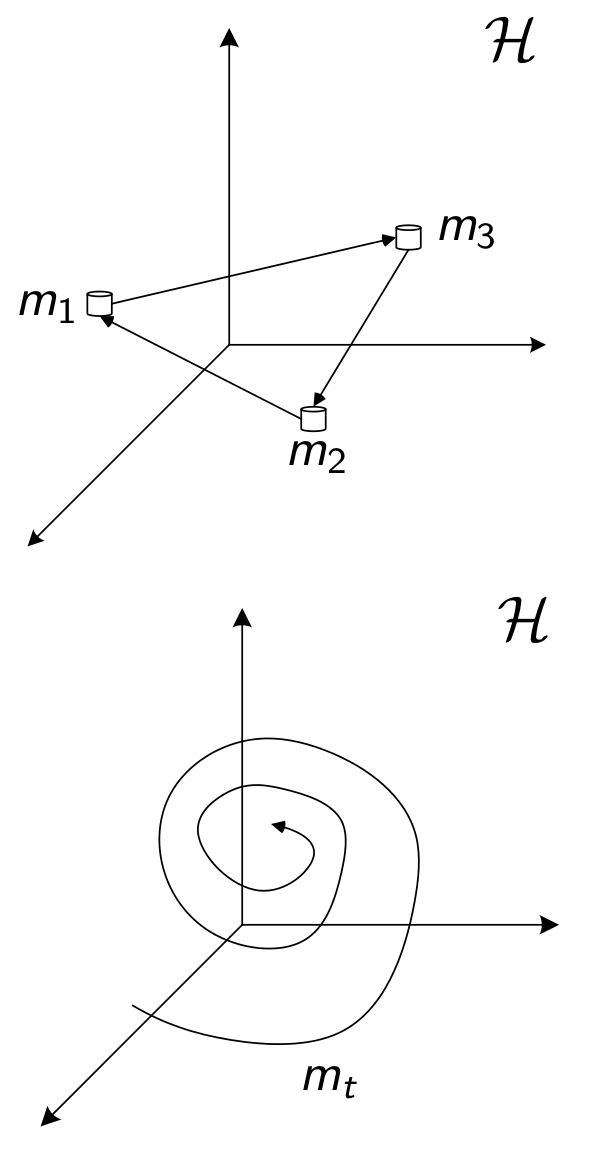
\includegraphics[height=1.0in]{Figure 3}
	\caption{\small{Two types of Hilbert space evolutions. Left: discrete switches in RKHS $\fspace$; Right: smooth evolution in $\fspace$.}}
	\label{fig:hilbert_evolution}           
	\end{minipage}\hfill

	\begin{minipage}{0.45\textwidth}
	\centering
	\subfloat[\small{1-shaded (Def. \ref{def:shaded})}]{
	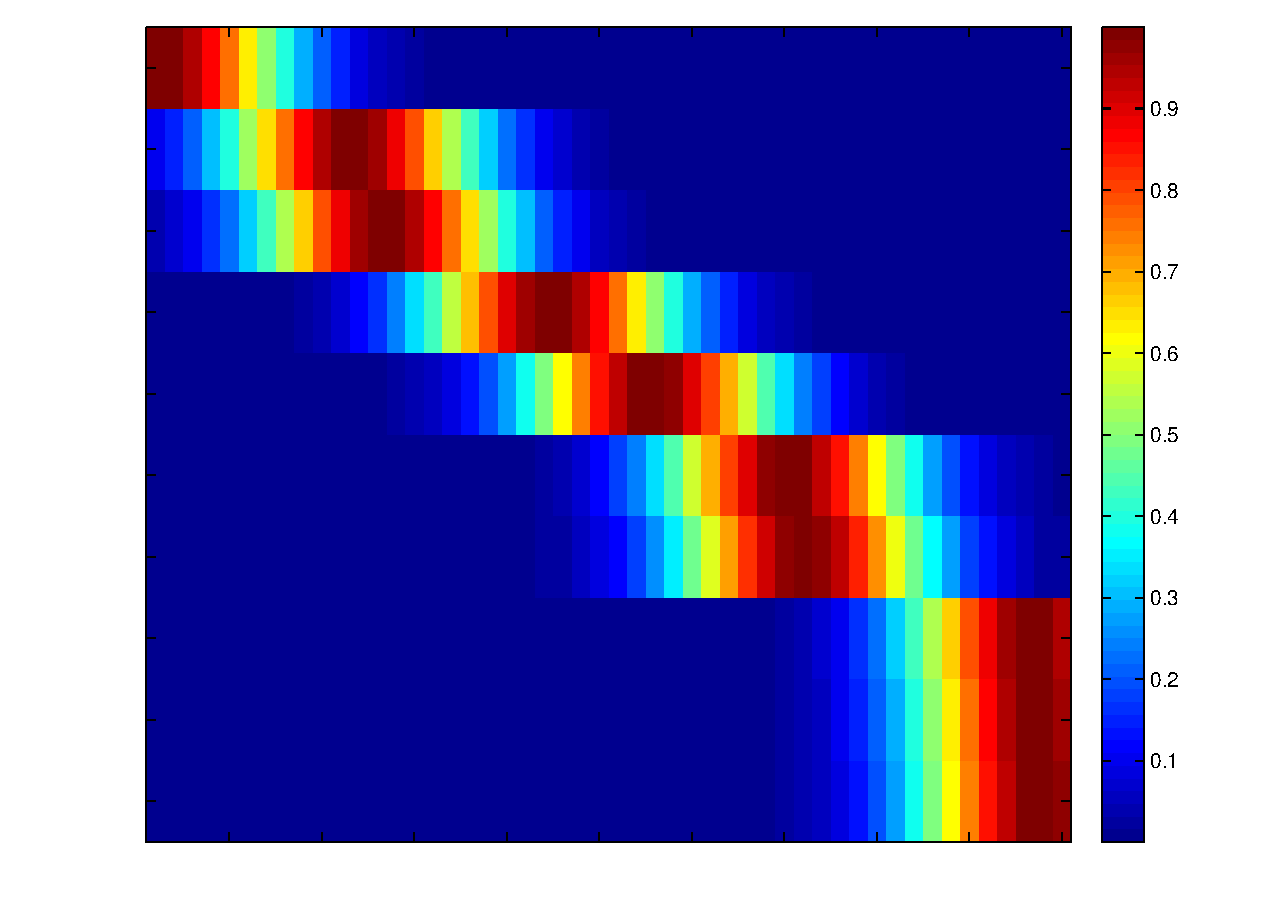
\includegraphics[width=0.47\columnwidth]{Figure 4a.pdf} \label{fig:shadeda}}
	\subfloat[\small{2-shaded (Eq. \eqref{empKShadFull})}]{
	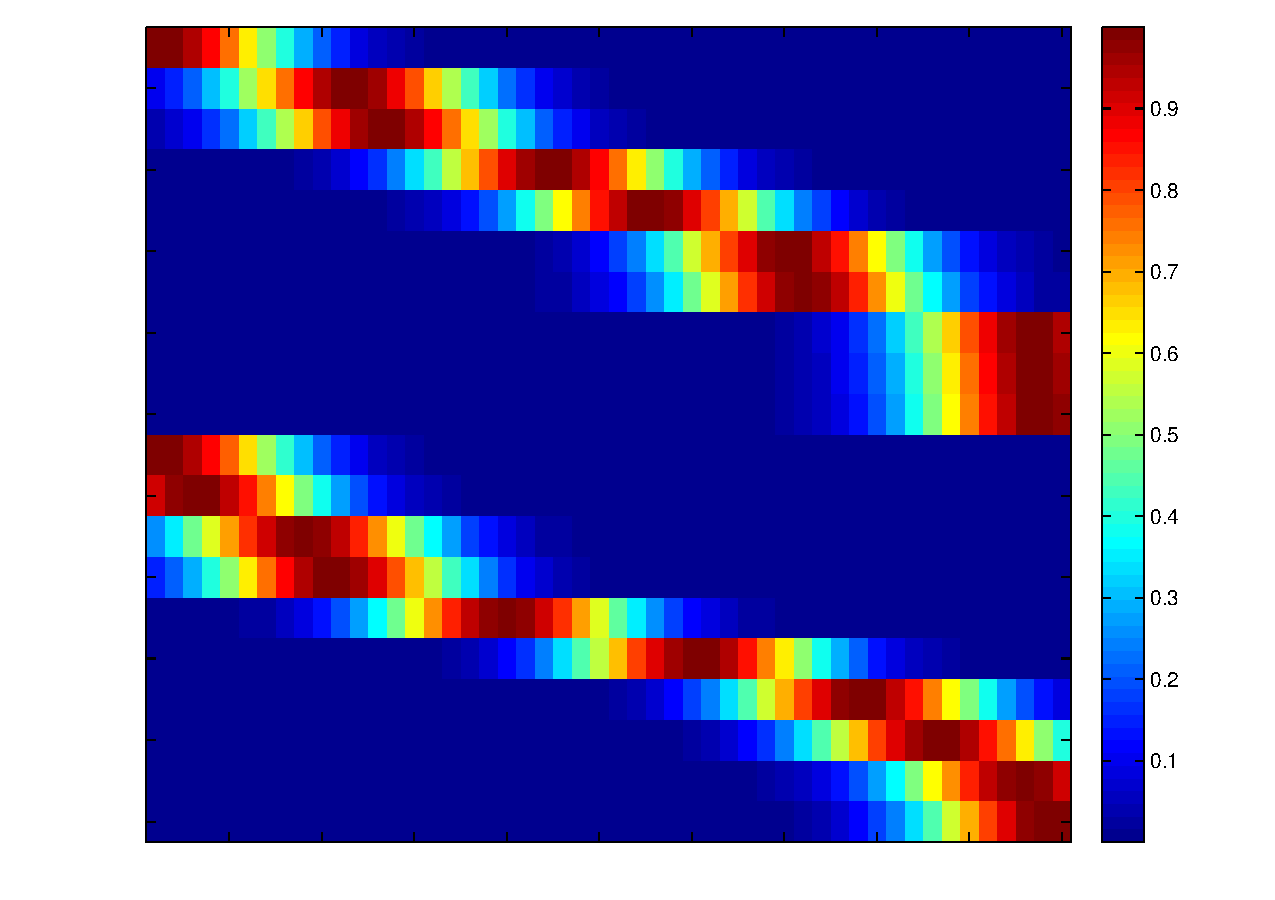
\includegraphics[width=0.47\columnwidth]{Figure 4b.pdf} \label{fig:shadedb}}
	\caption{\small{Shaded observation matrices for dictionary of atoms. Each row represents a sensing location with the color map indicating the evaluation of kernel function w.r.t the others points in the domain.}}
	\label{fig:shaded}
	\end{minipage}
\end{figure}


\begin{figure}[t]
\centering
\subfloat[\small{Gaussian}]{
 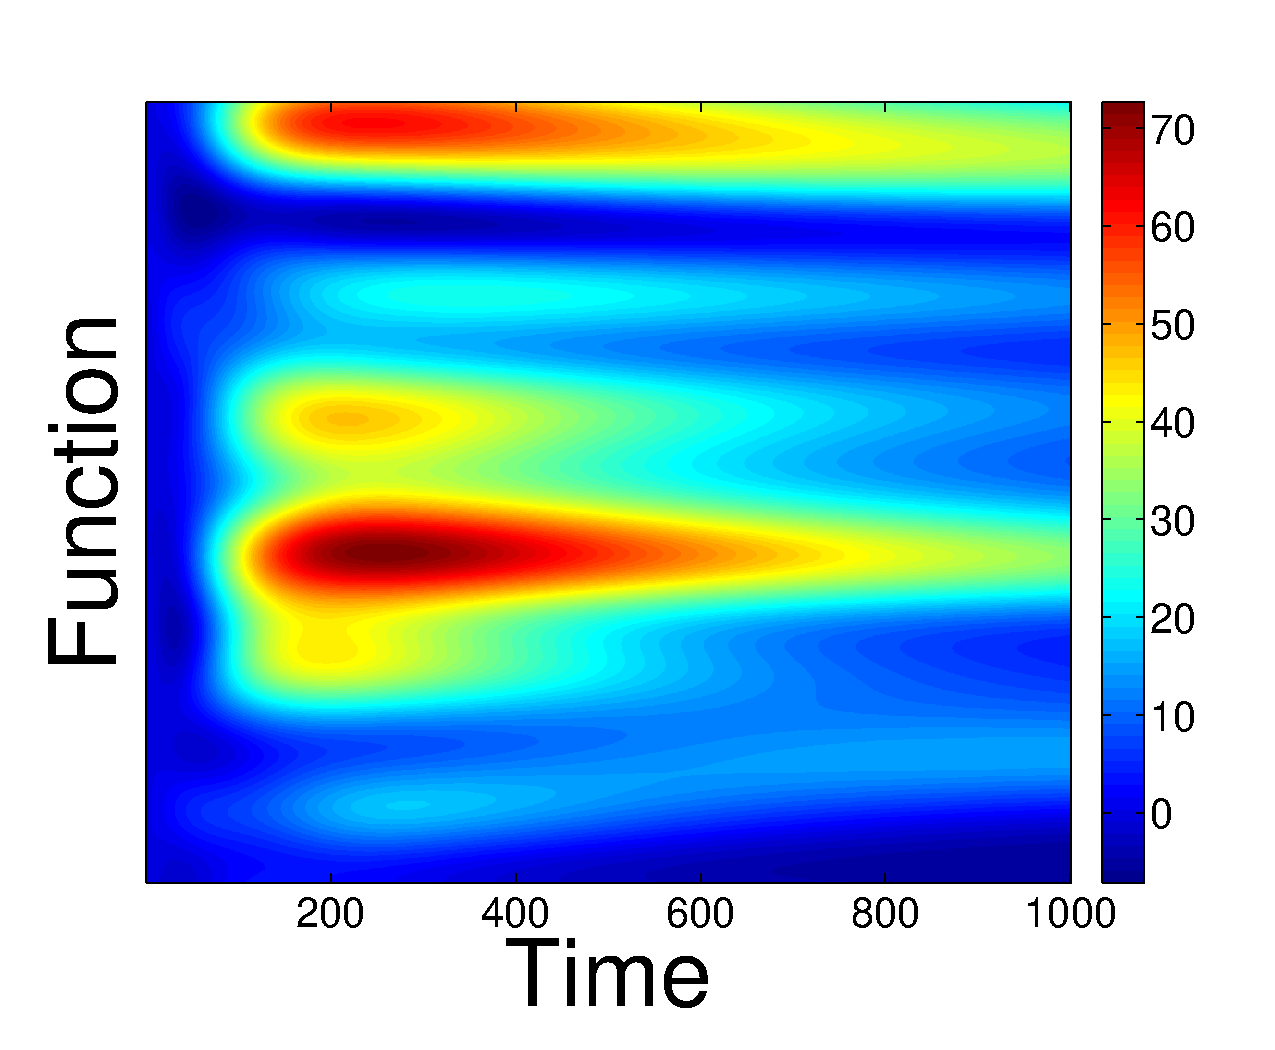
\includegraphics[width=0.25\columnwidth]{Figure 5a.pdf}
}
\subfloat[\small{Laplacian}]{
 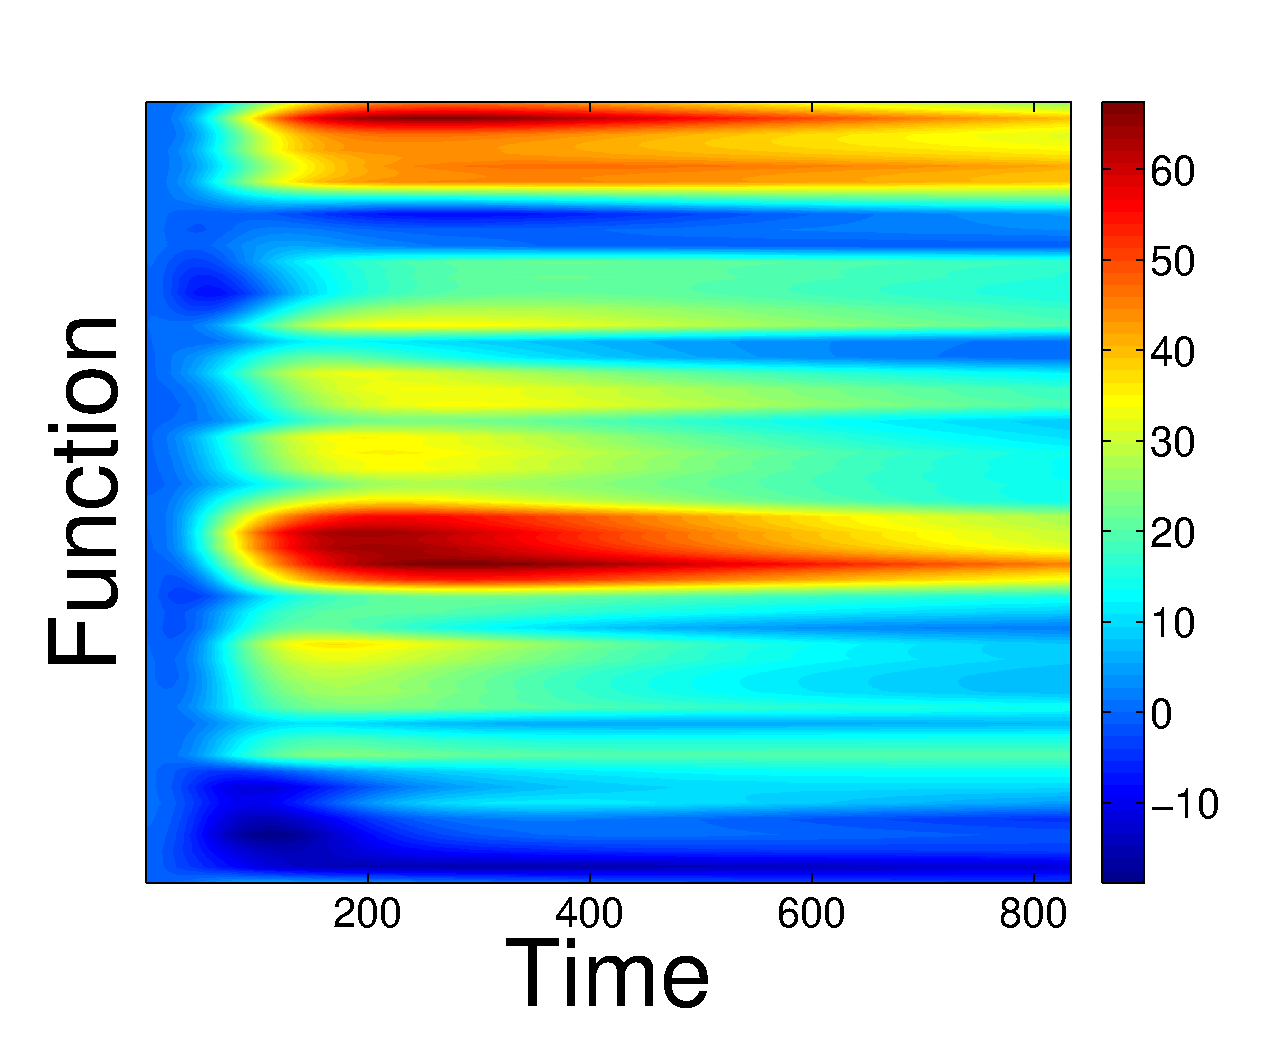
\includegraphics[width=0.25\columnwidth]{Figure 5b.pdf}
}
% \\
\subfloat[\small{Periodic}]{
 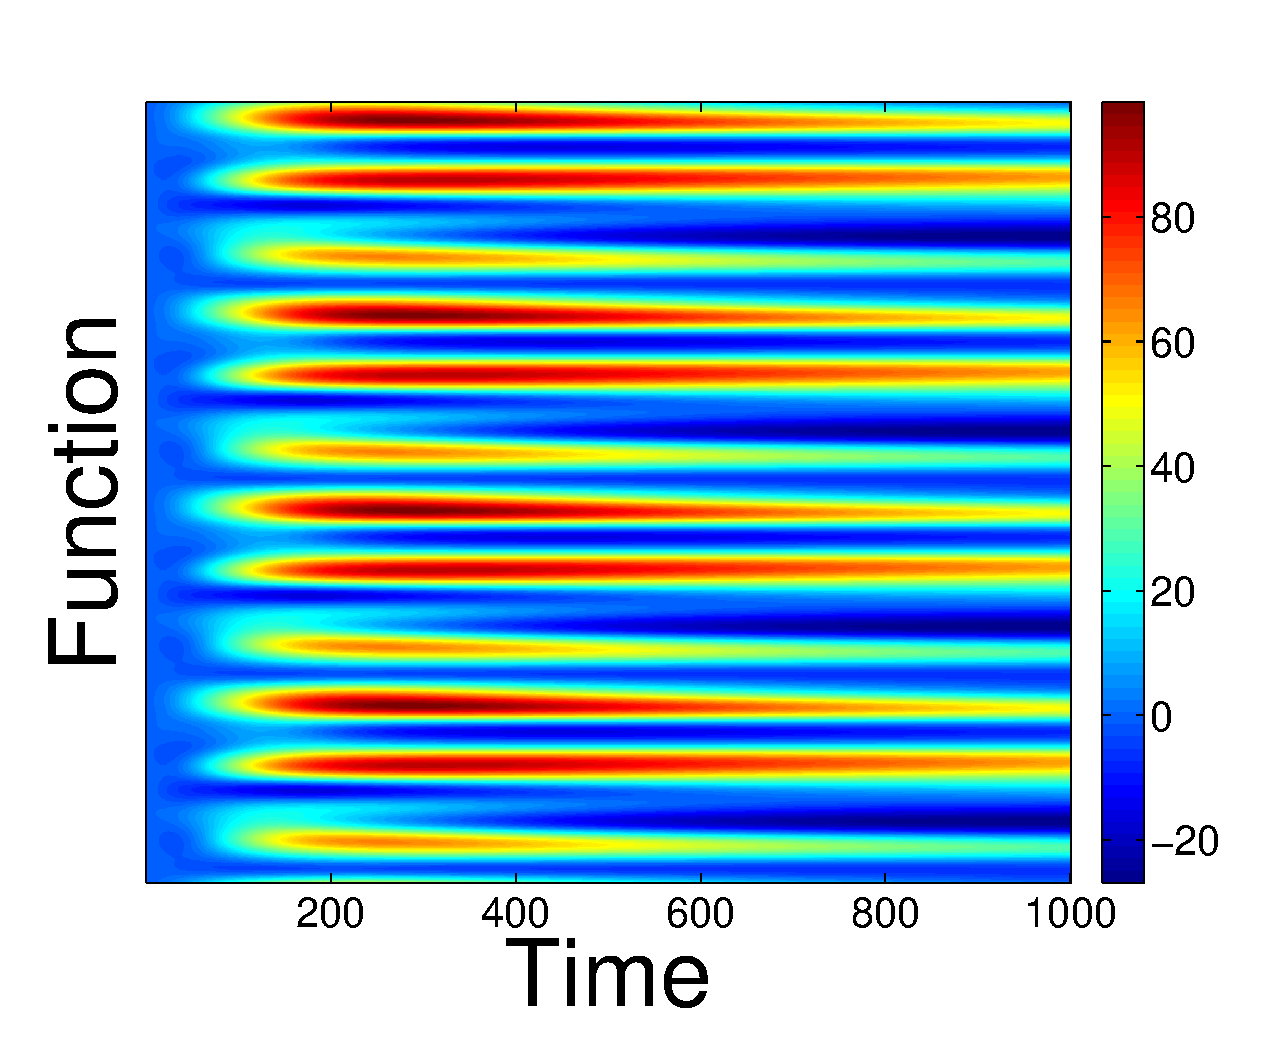
\includegraphics[width=0.25\columnwidth]{Figure 5c.pdf}
}
\caption{\small{One-dimensional function evolution over a fixed transition matrix $A$, 
initial condition $\weight_0$ and centers $\shCent$, but with different kernels $\kernel(x,y)$. 
Each $y$-vector at a given value of $x$ represents the output of the function, which evolves from left to right. 
As seen, changing the kernel creates quite different dynamic behaviors. }%behavior for the same system.}
}
\label{fig:kernel_variation}
\end{figure}


In this paper, we restrict our attention to the class of functional evolutions $\mathbb{F}$ defined by linear Markovian transitions in an RKHS. While extension to the nonlinear case is possible (and non-trivial), it is not pursued in this paper to help ease the exposition of the key ideas. The class of linear transitions in RKHS is rich enough to approximately model many real-world datasets, as suggested by our experiments.

Let $y\in\R^{\nsamp}$ be the measurements of the function available from $\nsamp$ sensors, $\sysop:\fspace\to\fspace$ be a linear transition operator in the RKHS $\fspace$, and $\measop:\fspace\to\R^{\nsamp}$ be a linear measurement operator. The model for the functional evolution and measurement studied in this paper is:
\begin{align}\eqlabel{ideal_lin_evol}
 f_{\tindex+1} = \sysop f_{\tindex} + \eta_{\tindex}, \quad
 y_{\tindex} = \measop_{\tindex} f_{\tindex} + \zeta_{\tindex},
\end{align}
where $\eta_{\tindex}$ is a zero-mean stochastic process in $\fspace$, and $\zeta_{\tindex}$ is a Wiener process in $\R^{\nsamp}$. 
Classical treatments of kernel methods emphasize that for most kernels, the feature map $\fmap$ is unknown, and possibly infinite-dimensional; this forces practioners to work in the dual space of $\fspace$, whose dimensionality is the number of samples in the dataset being modeled. This conventional wisdom precludes the use of kernel methods for most tasks involving modern datasets, which may have millions and sometimes billions of samples \cite{rahimi2007random}. An alternative is to work with a feature map 
$\fmapApprox(x) := \left[\begin{smallmatrix}
  \fmapApprox_1(x) & \cdots & \fmapApprox_{\ncent}(x)
 \end{smallmatrix}\right]^T$ to an approximate feature space
 $\fspaceApprox$ with the property that for every element $\fspaceEl\in\fspace$, $\exists\fspaceApproxEl\in\fspaceApprox$ s.t. $\|\fspaceEl-\fspaceApproxEl\| < \e$ for an appropriate function norm and $\e>0$. A few such approximations are listed below.
 
%\begin{enumerate}
\paragraph{Dictionary of atoms} Let $\dom$ be compact. Given points $\shCent = \shCentLong$, $c_i\in\dom$, we have a dictionary of atoms $\Atoms = \{\fmap(c_1), \cdots , \fmap(c_{\ncent})\}$, $\fmap(c_i)\in\fspace$, the span of which is a strict subspace $\fspaceApprox$ of the RKHS $\fspace$ generated by the kernel. Here, 
 \begin{equation}\eqlabel{fmap_dict}
 \fmapApprox_i(x) := \l\fmap(x), \fmap(c_i)\r_{\fspace} = \kernel(x, c_i).
 \end{equation}
\paragraph{Low-rank approximations} Let $\dom$ be compact, let $\shCent = \shCentLong$, $c_i\in\dom$, and let $\empK\in\R^{\ncent\times\ncent}$, $\empK_{ij}:=\kernel(c_i,c_j)$ be the Gram matrix computed from $\shCent$. This matrix can be diagonalized to compute approximations $(\empEval_i, \empEfunc_i(x))$ of the eigenvalues and eigenfunctions $(\eval_i, \efunc_i(x))$ of the kernel \cite{williams2001using2}. These spectral quantities can then be used to compute  $ \fmapApprox_i(x):=\sqrt{\empEval}_i\empEfunc_i(x)$.
 \paragraph{Random Fourier features} Let $\dom\subset\R^n$ be compact, and let $ \kernel(x,y) = e^{-\|x-y\|^2/2\s^2}$ be the Gaussian RBF kernel. Then random Fourier features approximate the kernel feature map as $\fmapApprox_{\randFreq}:\dom\to\fspaceApprox$, where $\randFreq$ is a sample from the Fourier transform of $\kernel(x,y)$, with the property that $\kernel(x,y) = \E_{\randFreq}[\l\fmapApprox_{\randFreq}(x),\fmapApprox_{\randFreq}(y)\r_{\fspaceApprox}]$ \cite{rahimi2007random}. In this case, if $\randMat\in\R^{M/2\times n}$ is a random matrix representing the sample $\randFreq$, then 
 $ 
  \fmapApprox_i(x) := \left[\begin{smallmatrix}
  \frac{1}{\sqrt{\ncent}}\sin([\randMat x]_i), \frac{1}{\sqrt{\ncent}}\cos([\randMat x]_i)
 \end{smallmatrix}\right]$. Similar approximations exist for other radially symmetric kernels, as well as dot-product kernels. 

\begin{figure}
	\centering
	
	\subfloat[Relationship between $\sysop$ and $A$]{
	\label{fig:commute_sysop_dyn}
	\begin{tikzpicture}
	  \matrix (m) [ampersand replacement=\&, matrix of math nodes, 
	                 row sep=0.75in,column sep=1in,minimum width=0.5in] {
	     \boldsymbol\fspaceApprox \& \boldsymbol\fspaceApprox \\
	     \pmb{\R^{\ncent}} \& \pmb{\R^{\ncent}} \\};
	  \path[-stealth]
	    (m-1-1) edge node [left] {$\boldsymbol\weightmap$} (m-2-1)
	            edge [right] node [above] {$\boldsymbol\sysop$} (m-1-2)
	    (m-2-1.east|-m-2-2) edge node [below] {$\boldsymbol A$} node [above] {} (m-2-2)
	    (m-2-2) edge node [right] {$\boldsymbol\weightmapI$} (m-1-2);            
	\end{tikzpicture}  
	}% end subfloat
	
	\subfloat[Relationship between $\measop$ and $\empK$]{
	\label{fig:commute_sysop_meas}
	
	\begin{tikzpicture}
	  \matrix (m) [ampersand replacement=\&, matrix of math nodes, 
	               row sep=0.75in,column sep=1in,minimum width=0.5in] {
	     \boldsymbol\fspaceApprox \& \pmb{\boldsymbol\R^{\nsamp}} \\
	     \pmb{\R^{\ncent}} \&  \\};
	  \path[-stealth]
	    (m-1-1) edge node [left] {$\boldsymbol\weightmap$} (m-2-1)
	            edge [right] node [above] {$\boldsymbol\measop$} (m-1-2)
	    (m-2-1) edge node [right] {$\ \boldsymbol\empK$} (m-1-2)
	    (m-2-1) edge node [right] {$\boldsymbol\weightmapI$} (m-1-1);            
	\end{tikzpicture}
	}% end subfloat
	
	\subfloat[Relationship between $\controlop$ and $B$]{
	\label{fig:commute_sysop_control}
	
	\begin{tikzpicture}
	  \matrix (m) [ampersand replacement=\&, matrix of math nodes, 
	                 row sep=0.75in,column sep=1in,minimum width=0.5in] {
	     \boldsymbol\fspaceD \& \boldsymbol\fspaceApprox \\
	     \pmb{\R^{\ncontrol}} \& \pmb{\R^{\ncent}} \\};
	  \path[-stealth]
	    (m-1-1) edge node [left] {$\boldsymbol\weightmapC$} (m-2-1)
	            edge [right] node [above] {$\boldsymbol\controlop$} (m-1-2)
	    (m-2-1.east|-m-2-2) edge node [below] {$\boldsymbol B$} node [above] {} (m-2-2)
	    (m-2-2) edge node [right] {$\boldsymbol\weightmapI$} (m-1-2);            
	\end{tikzpicture}
	}
	
	\caption{Commutative diagrams between primal and dual spaces}
	\vspace{-0.2in}
	\label{fig:commute_sysop}
\end{figure}



In the approximate space case, we replace the transition operator $\sysop:\fspace\to\fspace$ in \eqref{ideal_lin_evol} by $\sysopApprox:\fspaceApprox\to\fspaceApprox$.
This approximate regime, which combines the flexibility of a truly nonparametric approach with computational realizability, still allows for the representation of rich phenomena, as will be seen in the sequel, and in Figure \ref{fig:kernel_variation}. 
The finite-dimensional evolution equations approximating \eqref{ideal_lin_evol} in dual form are:
\vspace{-0.05in}
\begin{align} \eqlabel{k_measure}
 \weight_{\tindex+1} = \dualopApprox\weight_{\tindex} + \processnoise_{\tindex}, \quad 
 \meas_{\tindex} = \obsMat \weight_{\tindex} +\measnoise_{\tindex},
\end{align}
where we have matrices $\dualopApprox\in \R^{\ncent\times\ncent}, \ \obsMat\in \R^{\nsamp\times\ncent}$, the vectors $\weight_{\tindex}\in\R^{\ncent}$, and where we have slightly abused notation to let $\meas_{\tindex}, \processnoise_{\tindex}$ and $\measnoise_{\tindex}$ denote their $\fspaceApprox$ counterparts. Here $\obsMat$ is the matrix whose rows are of the form $\obsMat_{(i)} = \obsMatRow(x_i) =
 \left[\begin{smallmatrix}
  \fmapApprox_1(x_i) & \fmapApprox_2(x_i) & \cdots & \fmapApprox_{\ncent}(x_i)
 \end{smallmatrix}\right]$. In systems-theoretic language, each row of $\obsMat$ corresponds to a \emph{measurement} at a particular location, and the matrix itself acts as a measurement operator. 

The equations in \eqref{ideal_lin_evol} suggest an immediate extension to functional control problems. 
Pick another basis for $\fspace$ as $\cbasis(x) := \begin{bmatrix}\cbasis_1(x) &\cdots & \cbasis_{\ncontrol}(x)
\end{bmatrix}^T$, where the functions $\cbasis_j(x)$ are used to approximate the RKHS $\fspace$ generated by the kernel. We denote the span of these functions as $\fspaceD$. In the dictionary of atoms case, an example would be another set of atoms
 $\AtomsControl = \begin{bmatrix}\fmap(d_1) &\cdots & \fmap(d_{\ncontrol})
\end{bmatrix}$, $\fmap(d_j)\in\fspace$, $d_j\in\dom$, with $\fspaceD$ being a strict subspace of the RKHS $\fspace$  generated by the kernel. 
The functional evolution equation is then as follows:
\begin{align}\eqlabel{ideal_lin_evol_control}
 f_{\tindex+1} = \sysop f_{\tindex} + \controlop \control_{\tindex} + \eta_{\tindex}, \quad y_{\tindex} = \measop_{\tindex} f_{\tindex} + \zeta_{\tindex},
\end{align}
where the control functions $\control_{\tindex}$ evolve in $\fspaceD$, and $\controlop:\fspaceD\to\fspaceApprox$. To derive the finite-dimensional equivalent of $\controlop$, we have to work out the structure of the matrix $B$: since $\fspaceApprox$ is not, in general, isomorphic to $\fspaceD$, this imposes strict restrictions on $B$. We can derive $B$ using least squares using the inner product of $\fspace$. An instructive example is where both $\fspaceApprox$ and $\fspaceD$ are generated by dictionaries of atoms; recall that in this case, $\Atoms = 
 \begin{bmatrix}\fmap(c_1) &\cdots & \fmap(c_{\ncent})
\end{bmatrix}$ is the basis for $\fspaceApprox$, and let $\control = \sum_{j=1}^{\ncontrol}\weightc_j\fmap(d_j)$, and let $\Atoms = 
 \begin{bmatrix}\fmap(c_1) &\cdots & \fmap(c_{\ncent})
\end{bmatrix}$ be the basis for $\fspaceC$. Then the projection of $\delta$ onto $\fspaceApprox$ can be derived as: 


\begin{align}
 \begin{bmatrix}
  \l \delta, \fmap(c_1) \r_{\fspace}\\
   \vdots\\
  \l \delta, \fmap(c_{\ncent}) \r_{\fspace} 
 \end{bmatrix}
 = 
 \underbrace{
 \begin{bmatrix}
  \Kiprod{d_1}{c_1} & \cdots & \Kiprod{d_{\ncontrol}}{c_1}\\
   \vdots  &\ddots &\vdots\\
  \Kiprod{d_1}{c_{\ncent}} & \cdots & \Kiprod{d_{\ncontrol}}{c_{\ncent}}
 \end{bmatrix}}_{\empKCD}
  \begin{bmatrix}
   \weightc_1\\
   \vdots\\
   \weightc_{\ncontrol}
  \end{bmatrix}.
\end{align}

Note that in the dictionary of atoms case, the entries of $\empKCD$ can be computed in closed form as ${\empKCD}_{ij}:= \kernel(d_i, c_j)$,
using the reproducing property. 
This derivation shows that the operator $B$ is simply $\empKCD\in\R^{\ncent\times\ncontrol}$, the kernel matrix between the data $\centers$ generating the atoms $\Atoms$ of $\fspaceApprox$ and the data $\centerscontrol$ generating the atoms $\AtomsControl$ of $\fspaceD$. 

Thus, the finite-dimensional evolution equations equivalent to \eqref{ideal_lin_evol_control} are
\begin{align}
 \weight_{\tindex+1} = \dualopApprox\weight_{\tindex} + \empKCD\weightc_{\tindex}, \quad
 y_{\tindex} = \empK_{\tindex} w_{\tindex} \eqlabel{k_measure_c1}.
\end{align}
We define the \emph{generalized observability matrix} \cite{zhou:bk:96} as 
%\begin{align}\eqlabel{obs_mat}
$  \Obs_{\Tset} = 
 \left[
 \begin{smallmatrix}
  \empK \dualopApprox^{\tindex_1}\\
  \cdots\\
  \empK \dualopApprox^{\tindex_\otime}
 \end{smallmatrix}
 \right] $ 
%\end{align}
where $\Tset = \{\tindex_1, \dots, \tindex_{\otime}\}$ are the set of instances $\tindex_i$
when we apply the operator $\empK$. A linear system is said to be \emph{observable} if $\Obs_{\Tset}$ has full column rank (that is, $\mathrm{Rank} (\Obs_{\Tset})=\ncent$) for 
$\Tset = \{0, 1, \dots, \ncent-1\}$ \cite{zhou:bk:96}. Observability guarantees two critical facts: firstly, it guarantees that the state $\weight_0$ can be recovered exactly from a finite series of measurements $\{y_{{\tindex}_1}, y_{{\tindex}_2}, \dots, y_{{\tindex}_{\otime}}\}$; in particular, defining $y_{\Tset} = \begin{bmatrix}y_{{\tindex}_1}^T, y_{{\tindex}_2}^T, \cdots, y_{{\tindex}_{\otime}^T}\end{bmatrix}^T$, we have that $y_{\Tset} = \Obs_{\Tset}\weight_0.$  Secondly, it guarantees that a feedback based \emph{observer} can be designed such that the estimate of $\weight_{\tindex}$, denoted by $\estweight_{\tindex}$, converges exponentially fast to $\weight_{\tindex}$ in the limit of samples. Note that all our theoretical results assume $\dualopApprox$ is available: while we perform system identification in the experiments (\cite{Kingravi16_NIPS}), it is not the focus of the paper. 

We are now in a position to formally state the spatiotemporal modeling, control, and inference problems being considered: given a spatiotemporally evolving system modeled using \eqref{k_measure}, choose a set of $\nsamp$ sensing locations such that even with $\nsamp\ll \ncent$, the functional evolution of the spatiotemporal model can be estimated (which corresponds to \emph{monitoring}), can be predicted robustly (which corresponds to \emph{Bayesian filtering}), and which can be controlled (which corresponds to \emph{functional control}). Our approach to solve the monitoring and prediction problem relies on the design of the measurement operator $\empK$ so that the pair $(\empK, \dualopApprox)$ is observable: any Bayesian state estimator (for example a Kalman filter) utilizing this pair is denoted as a \textbf{kernel observer}. In the case where no measurements are taken, for the sake of consistency, we denote the state estimator as an \textit{autonomous} kernel observer. In the controls case, given a spatiotemporally evolving system modeled using \eqref{k_measure_c1}, we need to choose a set of $\nsamp$ sensing locations and $\ncontrol$ control locations, such that even with $\nsamp\ll \ncent, \ \ncontrol \ll\ncent$, the functional evolution of the spatiotemporal model can be controlled; in this case, we must design both a measurement operator $\empK$ and a control operator $\empKCD$ such that the pair $(\empKCD, \dualopApprox)$ is controllable: a controls system utilizing this pair and the measurement operator $\empK$ is denoted as a \textbf{kernel controller}.


\subsection{Preliminaries on Rational Canonical Structures}\label{sec_prelim}

We take a geometric approach towards the choice of sampling locations for inferring $\weight_{\tindex}$ in  \eqref{k_measure}; the extension for control is similar.  We use the notation $\linspace$, with $\dims(\linspace)=\ncent$, to emphasize the fact that these theorems hold for any finite-dimensional vector space. Consider the linear operator $\sysop:\linspace\rightarrow\linspace$, and recall that the definition of observability requires the construction of a linear operator $\measop:\linspace\to\linspaceout$, with $\dim(\linspaceout) = \nsamp$, such that 
$\Rank\left[
 \begin{smallmatrix}
  \left(\measop\right)^T &
  \cdots &
  \left(\measop \sysop^{\ncent-1}\right)^T
 \end{smallmatrix}
 \right]^T = \ncent$. 
In most applications, if $\nsamp\geq\ncent$, and $\Rank\left(\measop\right) = \nsamp$, it is reasonable to expect that observability may be achieved. However, for our purposes, $\nsamp$ must be \emph{significantly} less than $\ncent$. Therefore, we must design $\measop$ with as small a rank as possible. To do so, we require a series of vectors $\linvec_i$ that, under repeated iterations of $\sysop$, can generate a basis for $\linspace$. For this task, we will use a fundamental decomposition result from the theory of modules, known as the \emph{rational canonical structure} of $\sysop$ \cite{wonham1974linear}. The intuition here is that if the sequence $\{\linvec_i\}_{i}$ can generate this basis, it can be directly used to construct $\measop$.

The linear operator $\sysop:\linspace\rightarrow\linspace$ has a characteristic polynomial $\charpoly(\eval) $ such that $\charpoly(\sysop)=0 $ by the Cayley-Hamilton theorem. The minimal polynomial (MP) of $\sysop$ is the monic polynomial $\minpoly(\cdot)$ of least degree (denoted by $\degs(\cdot)$) given as 
$\minpoly(\eval) = \polycoeff_0 + \polycoeff_1\eval +\cdots + \eval^{\degs(\minpoly)} = 0$, such that
$\minpoly(\sysop)=\polycoeff_0 I + \polycoeff_1\sysop +\cdots + \sysop^{\degs(\minpoly)} = \bm{0}$. 
The MP is unique and divides $\charpoly(\lambda)$, so that $ \degs(\minpoly) \leq \degs(\charpoly)$. The MP of a vector $\linvec\in\linspace$ \emph{relative to $\sysop$} is the unique monic polynomial $\minpolyv_{\linvec}$ of least degree such that 
$\minpolyv_{\linvec}(\sysop)\linvec= \polycoeff_0\linvec + \polycoeff_1\sysop\linvec + \cdots + \sysop^{\degs(\minpoly)}\linvec = 0$. 
If $\degs(\alpha) = \ncent$, then $\sysop$ is \emph{cyclic} and $\exists\linvec\in \linspace$, such that the vectors $\{\linvec, \sysop \linvec,\dots,\sysop^{\ncent-1}\linvec\}$ form a basis for $\linspace$; this is the same as saying that the pair $(\linvec^T,\sysop^T)$ is observable.    
A subspace $\subspace\subset\linspace$ s.t. $\sysop\subspace\subset\subspace$ is \emph{$\sysop$-cyclic} if  $\restrict{\sysop}{\subspace}$, the restriction of $\sysop$ to the subspace $\subspace$, is cyclic. If $\minpoly(\eval)$ is the minimal polynomial of $\sysop$ and $\degs(\minpoly) = \acycdeg < \ncent$, $\exists~\linvec\in\linspace$ such that $\{\linvec, \sysop \linvec,\dots,\sysop^{\acycdeg-1}\linvec\}$ span an $\acycdeg$-dimensional $\sysop$-cyclic subspace $\subspace$, with $\linvec$ being the \emph{cyclic generator} of $\subspace$.  The subspace $\subspace$ decomposes $\linspace$ relative to $\sysop$. By the rational canonical structure theorem (Theorem 0.1 of \cite{wonham1974linear}), $\sysop$ can be successively decomposed into subspaces $\linspace_i \subset \linspace$, $i\in \{1,\dots,\minmeas\}$, s.t. $\linspace = \linspace_1 \oplus ... \oplus \linspace_{\minmeas}$, $\sysop\linspace_i \subset \linspace_i$, and  $\sysop_{|\linspace_i}, i \in \{1,\dots,\minmeas\}$, are cyclic. In general, the subspaces $\linspace_i$ are not unique for a fixed $\sysop$. The integer $\minmeas$ is unique and is called the \emph{cyclic index of $\sysop$}. 

One of our main results is to show that the cyclic index is a lower bound on the number of measurements required to reconstruct $\weight_{\tindex}$ (see Prop. \ref{prop:3} and Alg. 1 below). The matrix transform associated to this theorem is known as the \emph{Frobenius normal form} (denoted by $\FrobC\in\R^{\ncent\times\ncent}$ ): for $\sysop\in\R^{\ncent\times\ncent}$,  $\exists \FrobP\in\R^{\ncent\times\ncent}$ invertible  such that $\sysop = \FrobP\FrobC\FrobP^{-1}$. We will also use the \emph{Jordan decomposition}, where for $\sysop\in\R^{\ncent\times\ncent}$, $\exists \JorP\in\R^{\ncent\times\ncent}$ invertible such that $\sysop = \JorP\JorLa \JorP^{-1}$, where $\JorLa$ is a unique block diagonal matrix with Jordan blocks with $\eval_i$ along the diagonal. 
If all the eigenvalues $\eval_i$ are nonzero and real, we say the matrix has a \emph{full-rank Jordan decomposition}. 

